\thispagestyle{toanhocvadoisongnone}
\pagestyle{toanhocvadoisong}
\everymath{\color{toanhocdoisong}}
\graphicspath{{../toanhocdoisong/pic/}}
\blfootnote{$^1$\color{toanhocdoisong}Hà Nội.}
\begingroup
\AddToShipoutPicture*{\put(0,616){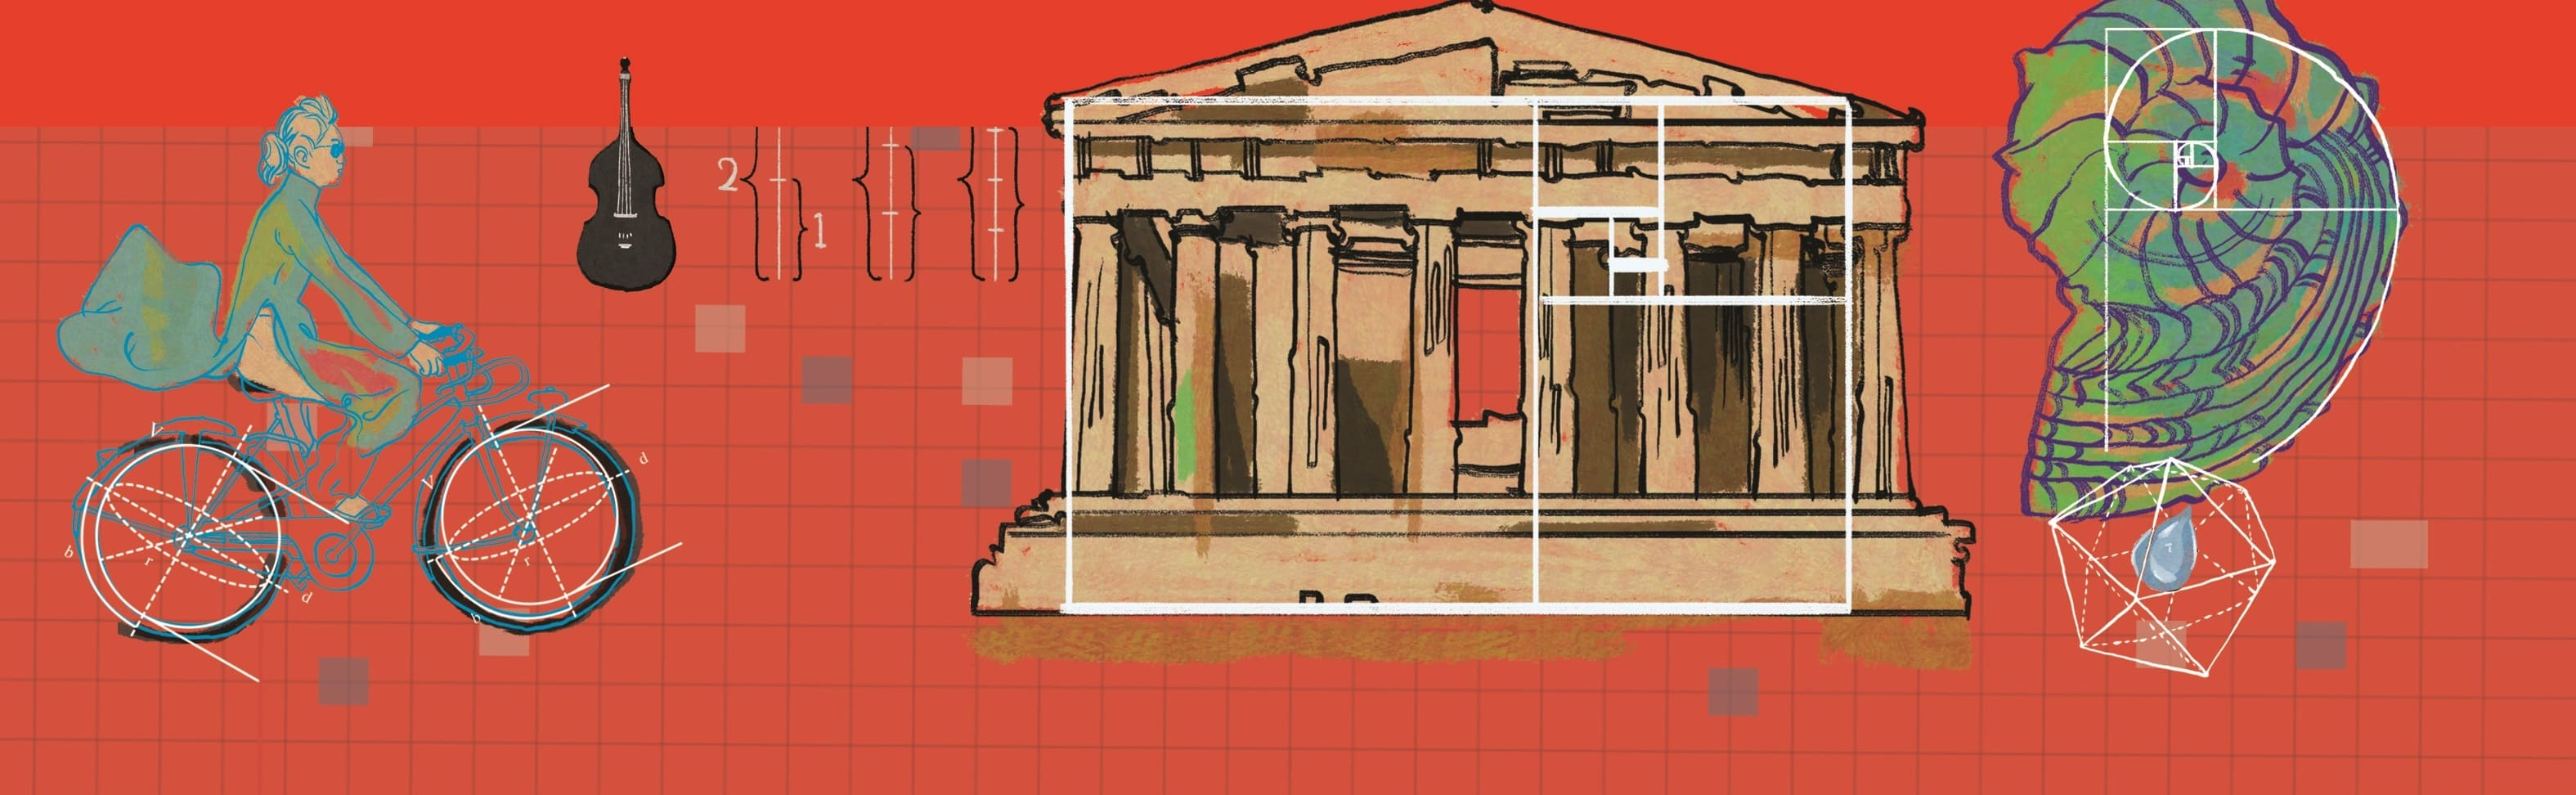
\includegraphics[width=19.3cm]{../bannertoanhocdoisong}}}
\AddToShipoutPicture*{\put(88,524){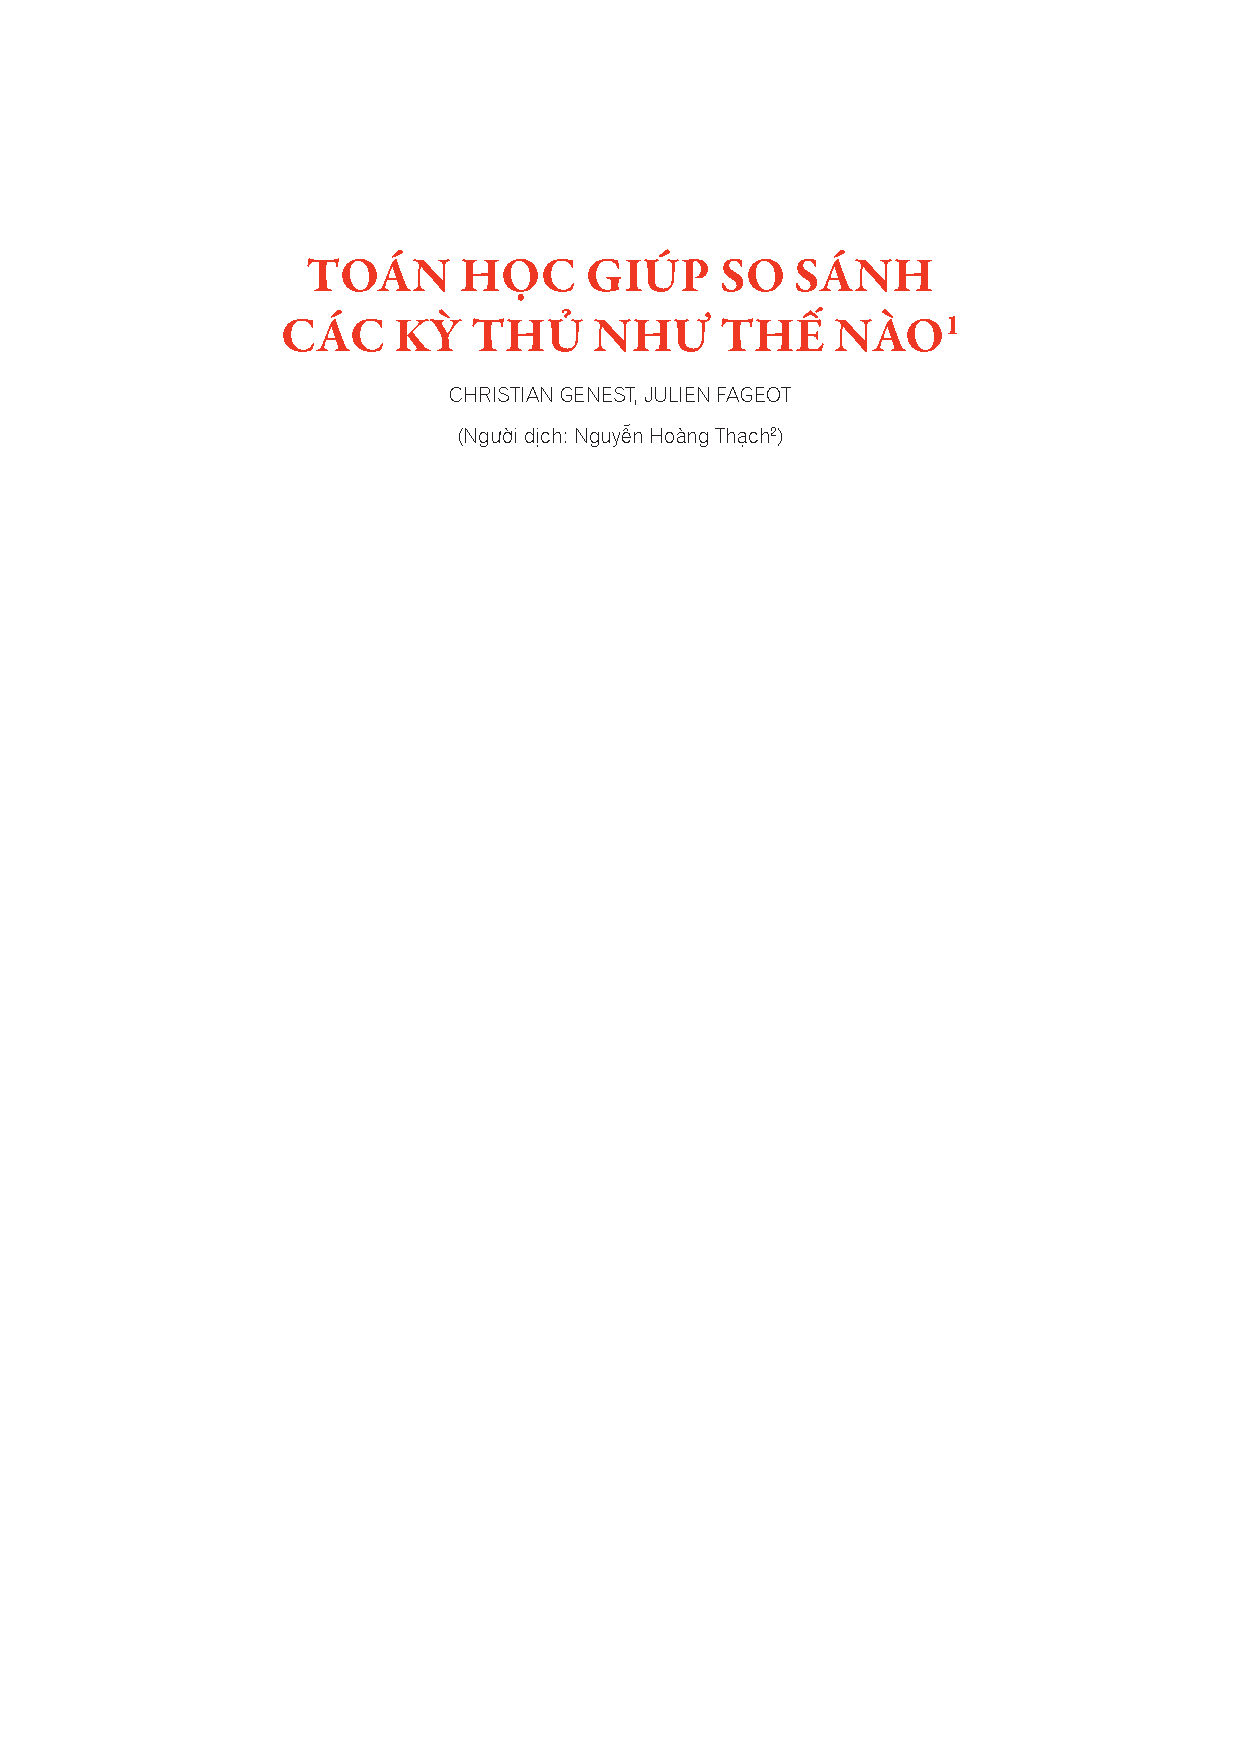
\includegraphics[scale=1]{../tieude.pdf}}}
\centering
\endgroup

\vspace*{182pt}

\begin{multicols}{2}
	Việc quản lý lượng hàng lưu trong kho là một vấn đề quan trọng trong thương nghiệp. Đây cũng là một bài toán cơ bản của ngành vận trù học. Trong bài viết này, chúng ta hãy cùng tìm hiểu một số mô hình toán học để tìm chi phí tối thiểu cho các tình huống khác nhau khi lưu trữ hàng trong kho.
	\vskip 0.1cm
	$\pmb{1.}$ \textbf{\color{toanhocdoisong}Ford Harris và mô hình EOQ cổ điển}
	\begin{figure}[H]
		\vspace*{-5pt}
		\centering
		\captionsetup{labelformat= empty, justification=centering}
		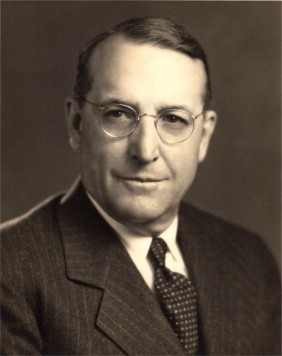
\includegraphics[width= 0.6\linewidth]{1}
		\caption{\small\textit{\color{toanhocdoisong}Ford Whitman Harris ($1877-1962$).}}
		\vspace*{-10pt}
	\end{figure}
	Mô hình EOQ (Economic Order Quantity) được Ford Whitman Harris, một kỹ sư lúc đó đang làm tư vấn về luật liên quan đến các bằng sáng chế, công bố năm $1913$. Đây là một mô hình đơn giản nhưng có tính thực tiễn cao về việc quản lý lượng hàng trong kho và vẫn có vai trò quan trọng trong ngành vận trù học ngày nay. 
	\vskip 0.1cm
	Mô hình EOQ này nhận các thông số đầu vào như sau:
	\vskip 0.1cm
	$K$: chi phí thiết lập cho một đơn hàng
	\vskip 0.1cm
	$c$: chi phí để sản xuất hoặc mua một đơn vị hàng
	\vskip 0.1cm
	$h$: chi phí để lưu một đơn vị hàng trong kho trong một đơn vị thời gian.
	\vskip 0.1cm
	Giả sử rằng nhu cầu tiêu thụ là đều theo thời gian và có giá trị $d$ đơn vị hàng/đơn vị thời gian. Nếu mỗi lần đặt hàng, ta đặt một lượng $Q$ đơn vị hàng thì số lượng hàng này sẽ được tiêu thụ hết trong thời gian $Q/d$. Chi phí cho một lần đặt hàng sẽ là $K+cQ$.
	\vskip 0.1cm
	Do lượng hàng sẽ giảm dần tuyến tính theo thời gian khi được bán ra, từ lúc nhận được $Q$ đơn vị hàng này đến khi tiêu thụ hết, số lượng đơn vị hàng trung bình được lưu trong kho từ đơn hàng này sẽ là $\dfrac{Q + 0}{2} = \dfrac{Q}{2}$. Chi phí lưu kho của đơn hàng cho đến khi bán hết sẽ là:
	\begin{align*}
		h\cdot \frac{Q}{2}\cdot \frac{Q}{d}=\frac{hQ^2}{2d}.
	\end{align*}
	Tổng chi phí cho một chu kỳ hàng sẽ là:
	\begin{align*}
		K + cQ + \frac{hQ^2}{2d}.
	\end{align*}
	Chi phí trong một đơn vị thời gian là:
	\begin{align*}
		T = \frac{K + cQ + \frac{hQ^2}{2d}}{\frac{Q}{d}} = \frac{dK}{Q} + dc + \frac{hQ}{2}.
	\end{align*}
	Ta cần tìm giá trị $Q^*$ sao cho $T$ nhận giá trị cực tiểu. Lấy đạo hàm của $T$ theo $Q$ được:
	\begin{align*}
		-\frac{dK}{Q^2} + \frac{h}{2} = 0.
	\end{align*}
	hay $Q^* = \sqrt{\dfrac{2dK}{h}}$.
	\vskip 0.1cm
	Nếu vẽ đồ thị của hàm $T(Q)$, ta được dạng đồ thị như trong Hình $1$. Hình dạng này của đồ thị hàm số có vai trò quan trọng trong một số bài toán ở các phần tiếp theo.
	\begin{figure}[H]
		\vspace*{-5pt}
		\centering
		\captionsetup{labelformat= empty, justification=centering}
		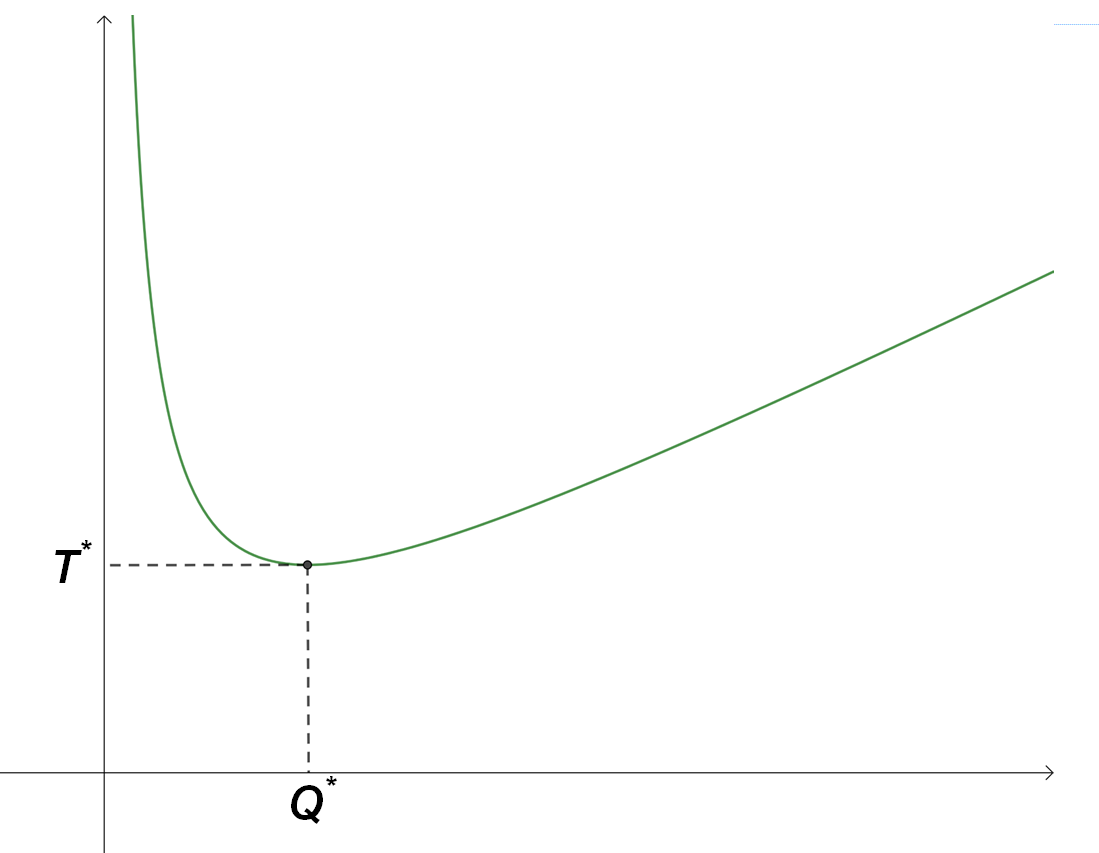
\includegraphics[width= 1\linewidth]{2}
		\caption{\small\textit{\color{toanhocdoisong}Hình $1$. Đồ thị của $T(Q)$.}}
		\vspace*{-10pt}
	\end{figure}
	Công thức EOQ dạng như trên xuất hiện ở nhiều giáo trình chuyên ngành kinh tế. Sau khi được Harris công bố năm $1913$, nó được nhiều tài liệu nhắc đến trong các thập kỷ sau đó (thường không có trích dẫn). Nhiều người gọi tên công thức này theo các tài liệu hoặc giáo trình mà họ biết. Vì lý do này, công thức EOQ còn được gọi là công thức Wilson hay công thức Camp. Trong khi đó, nguồn gốc từ Harris của công thức EOQ bị lãng quên cho đến khi được Donal Erlenkotter phát hiện lại vào năm $1988$. Một trong những nguyên nhân của vấn đề này có lẽ là do bản thân Harris không phải là một học giả. Tuy chỉ học hết cấp $3$, Harris đã tự phân đấu và học việc để trở thành một kỹ sư với nhiều bằng sáng chế. Sau đó, ông tiếp tục tự học và có một sự nghiệp thành công trong lĩnh vực luật về các bằng sáng chế. Bản thân Harris cũng không cố gắng đạt được sự công nhận cho công thức EOQ cho đến khi mất năm $1962$. Ông luôn cho rằng các sáng chế mang tính thực tiễn có giá trị hơn những ý tưởng trừu tượng.
	\vskip 0.1cm
	$\pmb{2.}$ \textbf{\color{toanhocdoisong}Mô hình EOQ có cho phép thiếu hụt}
	\vskip 0.1cm
	Trong thiết lập trên, ta chưa xét thời gian từ lúc đặt hàng cho đến khi hảng về kho. Trong thực tế, việc này không phải là ngay lập tức và việc sản xuất hoặc vận chuyển cần tốn một khoảng thời gian $L$ nào đó. Do đó, khi lượng hàng trong kho chi còn Ld (đủ dùng cho khoảng thời gian $L$) thì ta phải đặt lượng hàng $Q^*$.
	\begin{figure}[H]
		\vspace*{-5pt}
		\centering
		\captionsetup{labelformat= empty, justification=centering}
		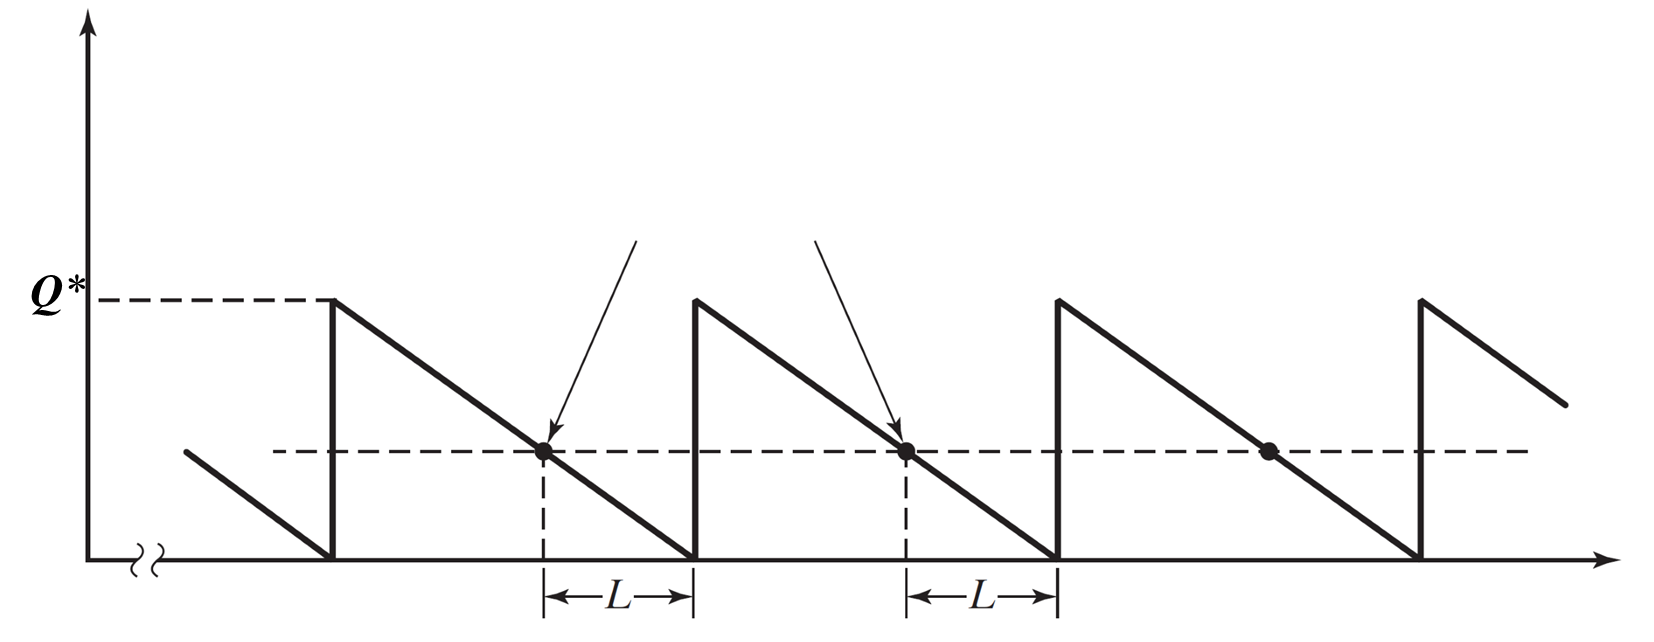
\includegraphics[width= 1\linewidth]{3}
		\caption{\small\textit{\color{toanhocdoisong}Hình $2$. Để tránh thiếu hụt, người ta cần đặt hàng khi lượng hàng còn lại trong kho đủ lớn sao cho trong khoảng thời gian này, thiếu hụt không xảy ra.}}
		\vspace*{-10pt}
	\end{figure}
	Mô hình này cũng có thể mở rộng trong trường hợp việc thiếu hụt là được cho phép. Nếu có nhu cầu cho hàng hóa mà hiện tại trong kho không có thì việc này được diễn tả bởi chi phí p, là chi phí phạt do thiếu hụt một đơn vị hàng trong một đơn vị thời gian. Trong thực tế, chi phí này có thể ứng với việc khách hàng mua hàng của công ty khác hoặc ta phải giảm giá cho khách hàng do họ phải đợi, ... Việc cân bằng giữa chi phí phạt do thiếu hụt và chi phí lưu hàng cho kho sẽ cho ta phương án với chi phí thấp nhất.
	\vskip 0.1cm
	Giả sử mỗi lần đặt hàng có lượng hàng là $Q$. Do có sự thiếu hụt nên sau khi giải quyết hết thiếu hụt, lượng hàng vào kho sẽ là $S$. Lượng hàng chịu chi phí do thiếu hụt sẽ là $Q-S$. Trong một chu kỳ thời gian $\dfrac{Q}{d}$, khoảng thời gian $\dfrac{S}{d}$ ban đầu sẽ không có thiếu hụt nhưng có chi phí lưu hàng trong kho còn khoảng thời gian còn lại không có hàng lưu kho.
	\begin{figure}[H]
		\vspace*{-5pt}
		\centering
		\captionsetup{labelformat= empty, justification=centering}
		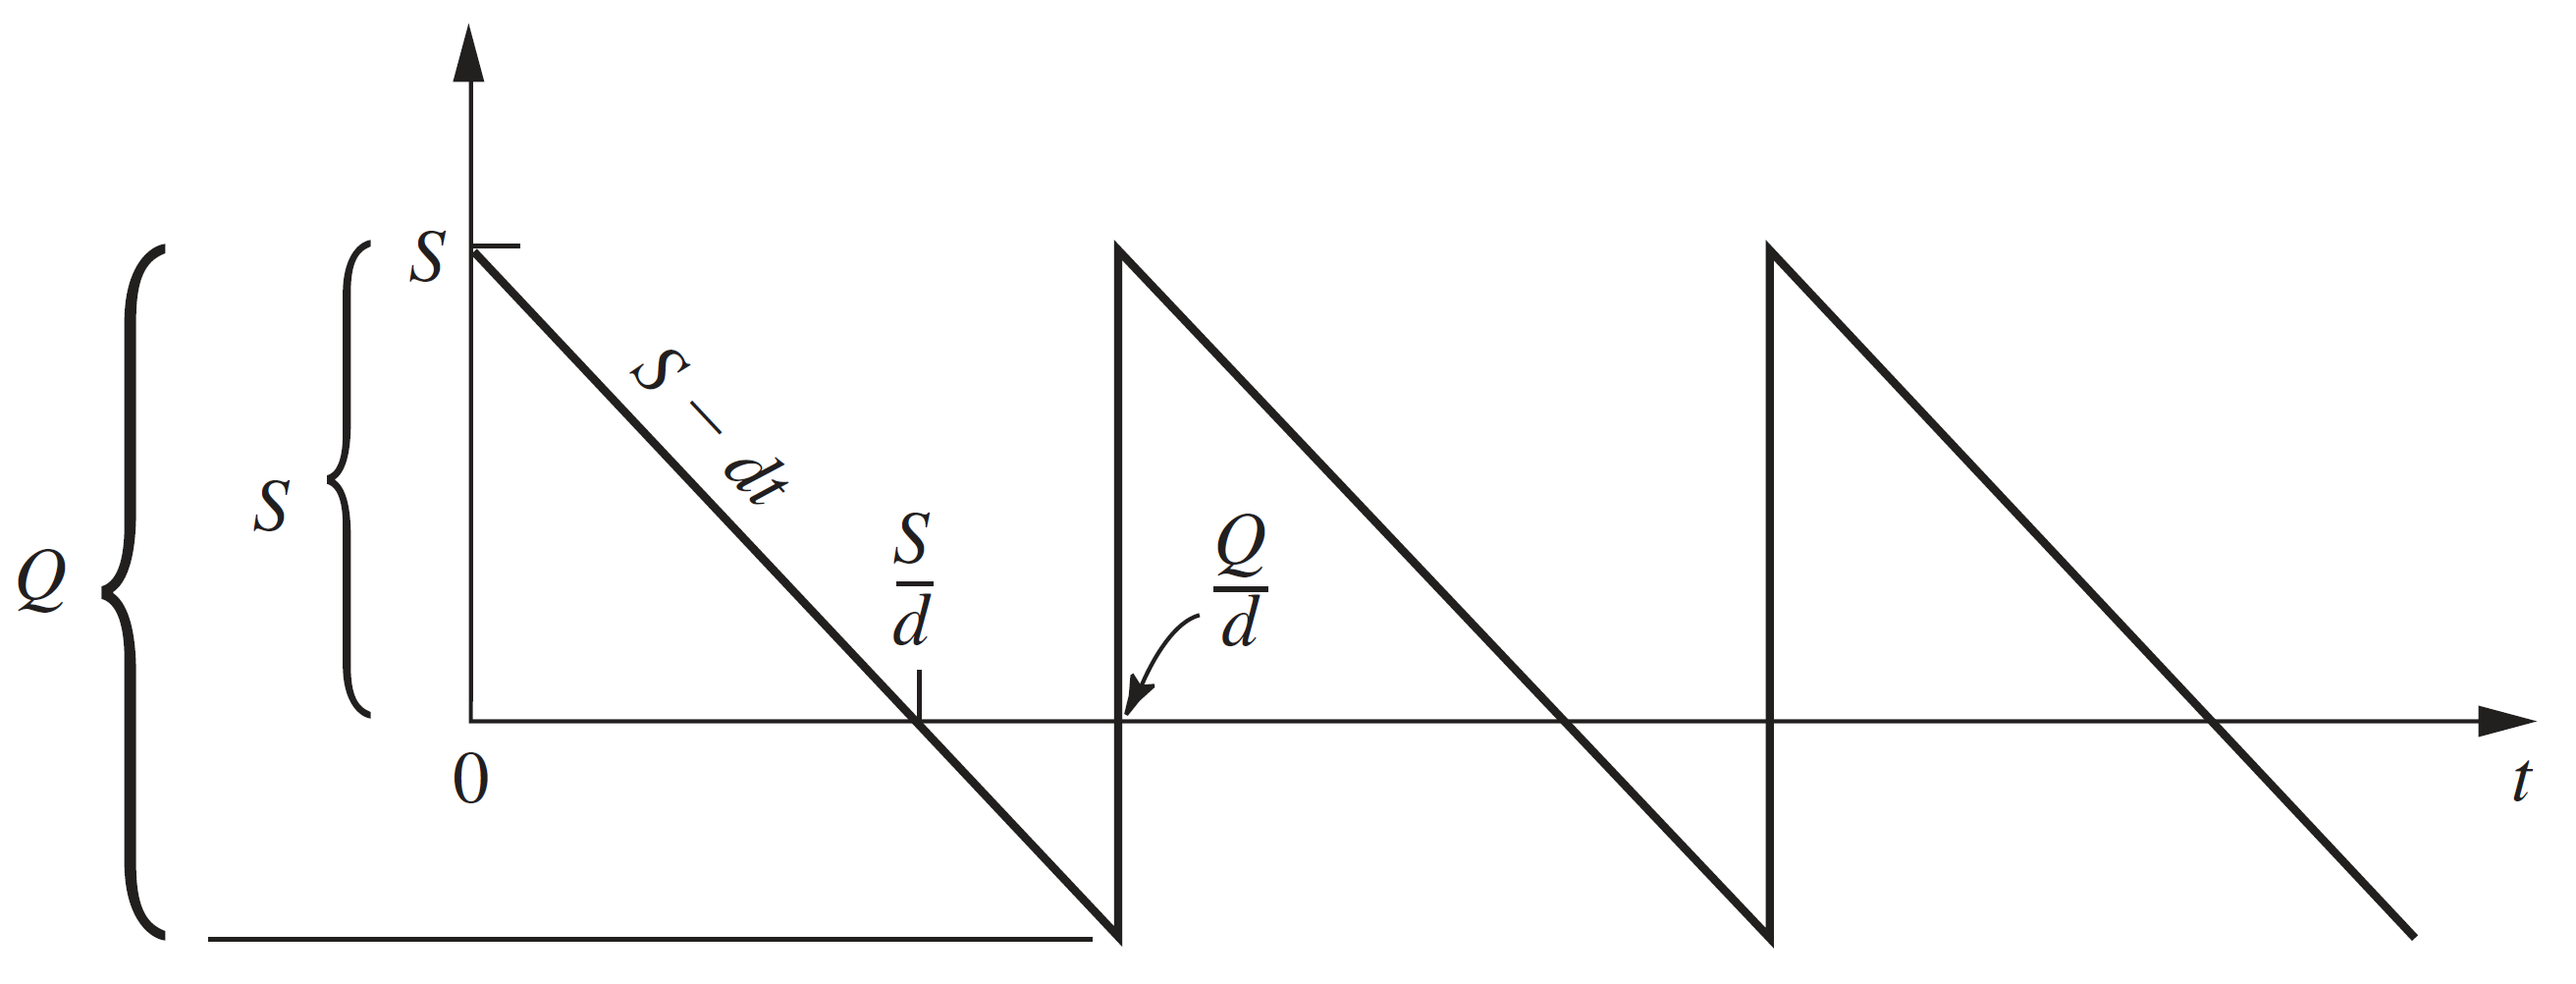
\includegraphics[width= 1\linewidth]{4}
		\caption{\small\textit{\color{toanhocdoisong}Hình $3$. Mô hình $EOQ$ có cho phép thiếu hụt xảy ra.}}
		\vspace*{-10pt}
	\end{figure}
	Tương tự với phần trên, chi phí đặt hàng vẫn là $K+cQ$ nhưng chi phí lưu kho trong một chu kỳ sẽ là
	\begin{align*}
		h\cdot\frac{S}{2}\cdot\frac{S}{d} = \frac{hS^2}{2d}.
	\end{align*}
	Trong khoảng thời gian thiếu hụt, lượng thiếu hụt trung bình sẽ là $\dfrac{Q-S}{2}$ nên chi phí phát sinh do thiếu hụt trong một chu kỳ sẽ là:
	\begin{align*}
		p\cdot\frac{Q-S}{2}\cdot\frac{Q-S}{d} = \frac{p(Q-S)^2}{2d}.
	\end{align*}
	Tổng chi phí trong một chu kỳ sẽ là:
	\begin{align*}
		K + cQ + \frac{hS^2}{2d} + \frac{p(Q-S)^2}{2d}.
	\end{align*}
	Tổng chi phí trong một đơn vị thời gian là:
	\begin{align*}
		T &= \frac{K + cQ + \frac{hS^2}{2d} + \frac{p(Q-S)^2}{2d}}{\frac{Q}{d}}\\
		 &= \frac{Kd}{Q} + cd + \frac{hS^2}{2Q} + \frac{p(Q-S)^2}{2Q}.
	\end{align*}
	Trong trường hợp này, cả $Q$ và $S$ đều thay đổi được nên $T$ là một hàm số của cả $Q$ lẫn $S$. Đây là một hàm số nhiều biến chứ không phải hàm số một biến như trong toán phổ thông. Vậy phải làm sao để tìm giá trị của $Q$ và $S$ để $T$ cực tiểu?
	\vskip 0.1cm
	Cần nhớ lại rằng, với hàm số một biến dạng $y=f(x)$ thì đạo hàm $\dfrac{dy}{dx}$ cho ta biết tốc độ biến thiên của $y$ khi $x$ thay đổi. Với những hàm số nhiều biến, để biểu diễn tốc độ biến thiên của nó khi một trong các biến thay đổi, người ta sử dụng khái niệm đạo hàm riêng. Đạo hàm riêng được tính cho từng biến. Trong trường hợp $T$, nó là hàm số $T(Q,S)$ của cả hai biến $Q$ và $S$ nên ta có hai đạo riêng, một cho $Q$ (ký hiệu $\dfrac{\partial T}{\partial Q}$) và một cho $S$ (ký hiệu $\dfrac{\partial T}{\partial S}$) . Việc tính đạo hàm riêng cũng không khác là mấy so với tính đạo hàm của hàm số một biến. Khi lấy đạo hàm riêng theo một biến, ta coi các biến còn lại không đổi và áp dụng các quy tắc giống như khi lấy đạo hàm của hàm số một biến.
	\vskip 0.1cm
	Trong trường hợp hàm $T(Q,S)$, ta có:
	\begin{align*}
		&\frac{\partial T}{\partial S} = \frac{hS}{Q} - \frac{p(Q-S)}{Q},\\
		&\frac{\partial T}{\partial Q} = \!- \frac{dK}{Q^2} \!-\! \frac{hS^2}{2Q^2} \!+\! \frac{p(Q\!-\!S)}{Q} \!-\! \frac{p(Q\!-\!S)^2}{2Q^2}.
	\end{align*}
	Để tìm cực trị của hàm nhiều biến, ta tìm điểm mà tại đó các đạo hàm riêng của nó bằng $0$ (tương tự như việc dùng đạo hàm để tìm cực trị của hàm số một biến). Với $T$, điều kiện này tương đương với hệ phương trình:
	\begin{align*}
		\begin{cases}
			\frac{hS}{Q} - \frac{p(Q-S)}{Q}= 0\\
			\!-\!\frac{dK}{Q^2} \!-\! \frac{hS^2}{2Q^2} \!+\! \frac{p(Q\!-\!S)}{Q} \!-\! \frac{p(Q\!-\!S)^2}{2Q^2}\!=\! 0.
		\end{cases}
	\end{align*}
	Hệ phương trình này tương đương với:
	\begin{align*}
		\begin{cases}
			S = \frac{p}{p+h}Q\\
			\!-\!dK \!-\! \frac{hS^2}{2} \!+\! p(Q-S)Q \!-\! \frac{p}{2}(Q\!-\!S)^2 \!=\! 0
		\end{cases}
	\end{align*}
	Tiến hành thế sử dụng biểu thức của $S$ theo $Q$ ta có:
	\begin{align*}
		&-dK \!-\! \frac{h}{2}\left(\!\!\frac{p}{p+h}\!\!\right)^2Q^2 \!+\! p\left(\!\!Q \!-\! \frac{p}{p+h}Q\!\right)\!Q \\
		&- \frac{p}{2}\left(Q - \frac{p}{p+h}Q\right)^2 = 0\\
		&-dK - \frac{h}{2}\left(\frac{p}{p+h}\right)^2Q^2 + \frac{ph}{p+h}Q^2 \\
		&- \frac{ph^2}{2(p+h)^2}Q^2 = 0\\
		&\frac{1}{2}\frac{\left(-p^2h + 2ph(p+h)-ph^2\right)}{(p+h)^2}Q^2 = dK\\
		&\frac{1}{2}\cdot\frac{ph(p+h)}{(p+h)^2}Q^2 = dK\\
		&Q^2 = \frac{2dK}{h}\cdot\frac{p+h}{p}.
	\end{align*}
	Ta được các giá trị của $S$ và $Q$ tại điểm cực trị:
	\begin{align*}
		Q^*\!=\!\sqrt{\frac{2dK}{h}}\sqrt{\!\frac{p+h}{p}},S^*\!=\! \sqrt{\!\frac{2dK}{h}}\sqrt{\!\frac{p}{p+h}}.
	\end{align*}
	Khi đó, chu kỳ tối ưu của việc đặt hàng sẽ là:
	\begin{align*}
		t^* = \frac{Q^*}{d}= \sqrt{\dfrac{2K}{dh}}\sqrt{\dfrac{p+h}{p}}.
	\end{align*}
	Số đơn vị hàng có tình trạng thiếu sẽ là:
	\begin{align*}
		Q^*- S^* = \sqrt{\dfrac{2dK}{p}}\sqrt{\dfrac{h}{p+h}}.
	\end{align*}
	Chính sách nhập hàng của ta sẽ thay đổi theo các giá trị của $h$ và $p$. Khi $p \to \infty$ còn $h$ không đổi, $Q^*-S^* \to 0$ và ta trở lại mô hình EOQ cơ bản: chi phí thiệt hại khi có thiếu hụt là quá lớn nên việc thiếu hụt không được phép xảy ra. Ngược lại, nếu $h \to \infty$ với $p$ không đổi (chi phí giữ hàng trong kho rất lớn so với thiệt hại do thiếu hụt), thì $S^* \to 0$ hay việc sử dụng kho hàng là không khả thi về mặt kinh tế và tất cả các nhu cầu mua hàng đều không được đáp ứng ngay mà được gom lại và giải quyết theo từng đợt mà không có lưu kho.
	\vskip 0.1cm
	$\pmb{3}$ \textbf{\color{toanhocdoisong}Mô hình EOQ với giá thành phân tầng}
	\vskip 0.1cm
	Ta hãy xử lý một tình huống khá thú vị xuất phát từ thực tế. Khi đặt hàng, nếu số lượng hàng vượt quá một ngưỡng $q$ nào đó, giá mua vào có thể được chiết khấu giảm đi. Ta hãy xét hàm chi phí mua vào cho một đơn vị hàng như sau:
	\begin{align*}
		c(Q)= \begin{cases}
			c_1,Q <q\\
			c_2,Q \ge q
		\end{cases}
	\end{align*}
	với $c_2<c_1$.
	\vskip 0.1cm
	Ta được hai hàm chi phí ứng với hai giá mua này (để đơn giản, trường hợp có thiếu hụt không được cho phép):
	\begin{align*}
		T_1 = \dfrac{dK}{Q} + c_1d  + \frac{hQ}{2},\\
		T_2 = \frac{dK}{Q} + c_2d + \frac{hQ}{2}.
	\end{align*}
	$T_2$ có hình dạng đồ thị giống hệt $T_1$ nhưng được tịnh tiến xuống một khoảng $(c_1-c_2 )d$ theo trục $y$. Hai đồ thị này đều có giá trị cực tiểu tại $Q=Q^*$. Ta cần chú ý đến điểm $Q_1>Q^*$ có $T_1 (Q_1 )=T_2 (Q^*)$ và dùng điểm này để biện luận các trường hợp (bạn đọc có thể tự giải để tìm $Q_1$, nó sẽ là nghiệm của một phương trình bậc hai).
	\begin{figure}[H]
		\vspace*{-5pt}
		\centering
		\captionsetup{labelformat= empty, justification=centering}
		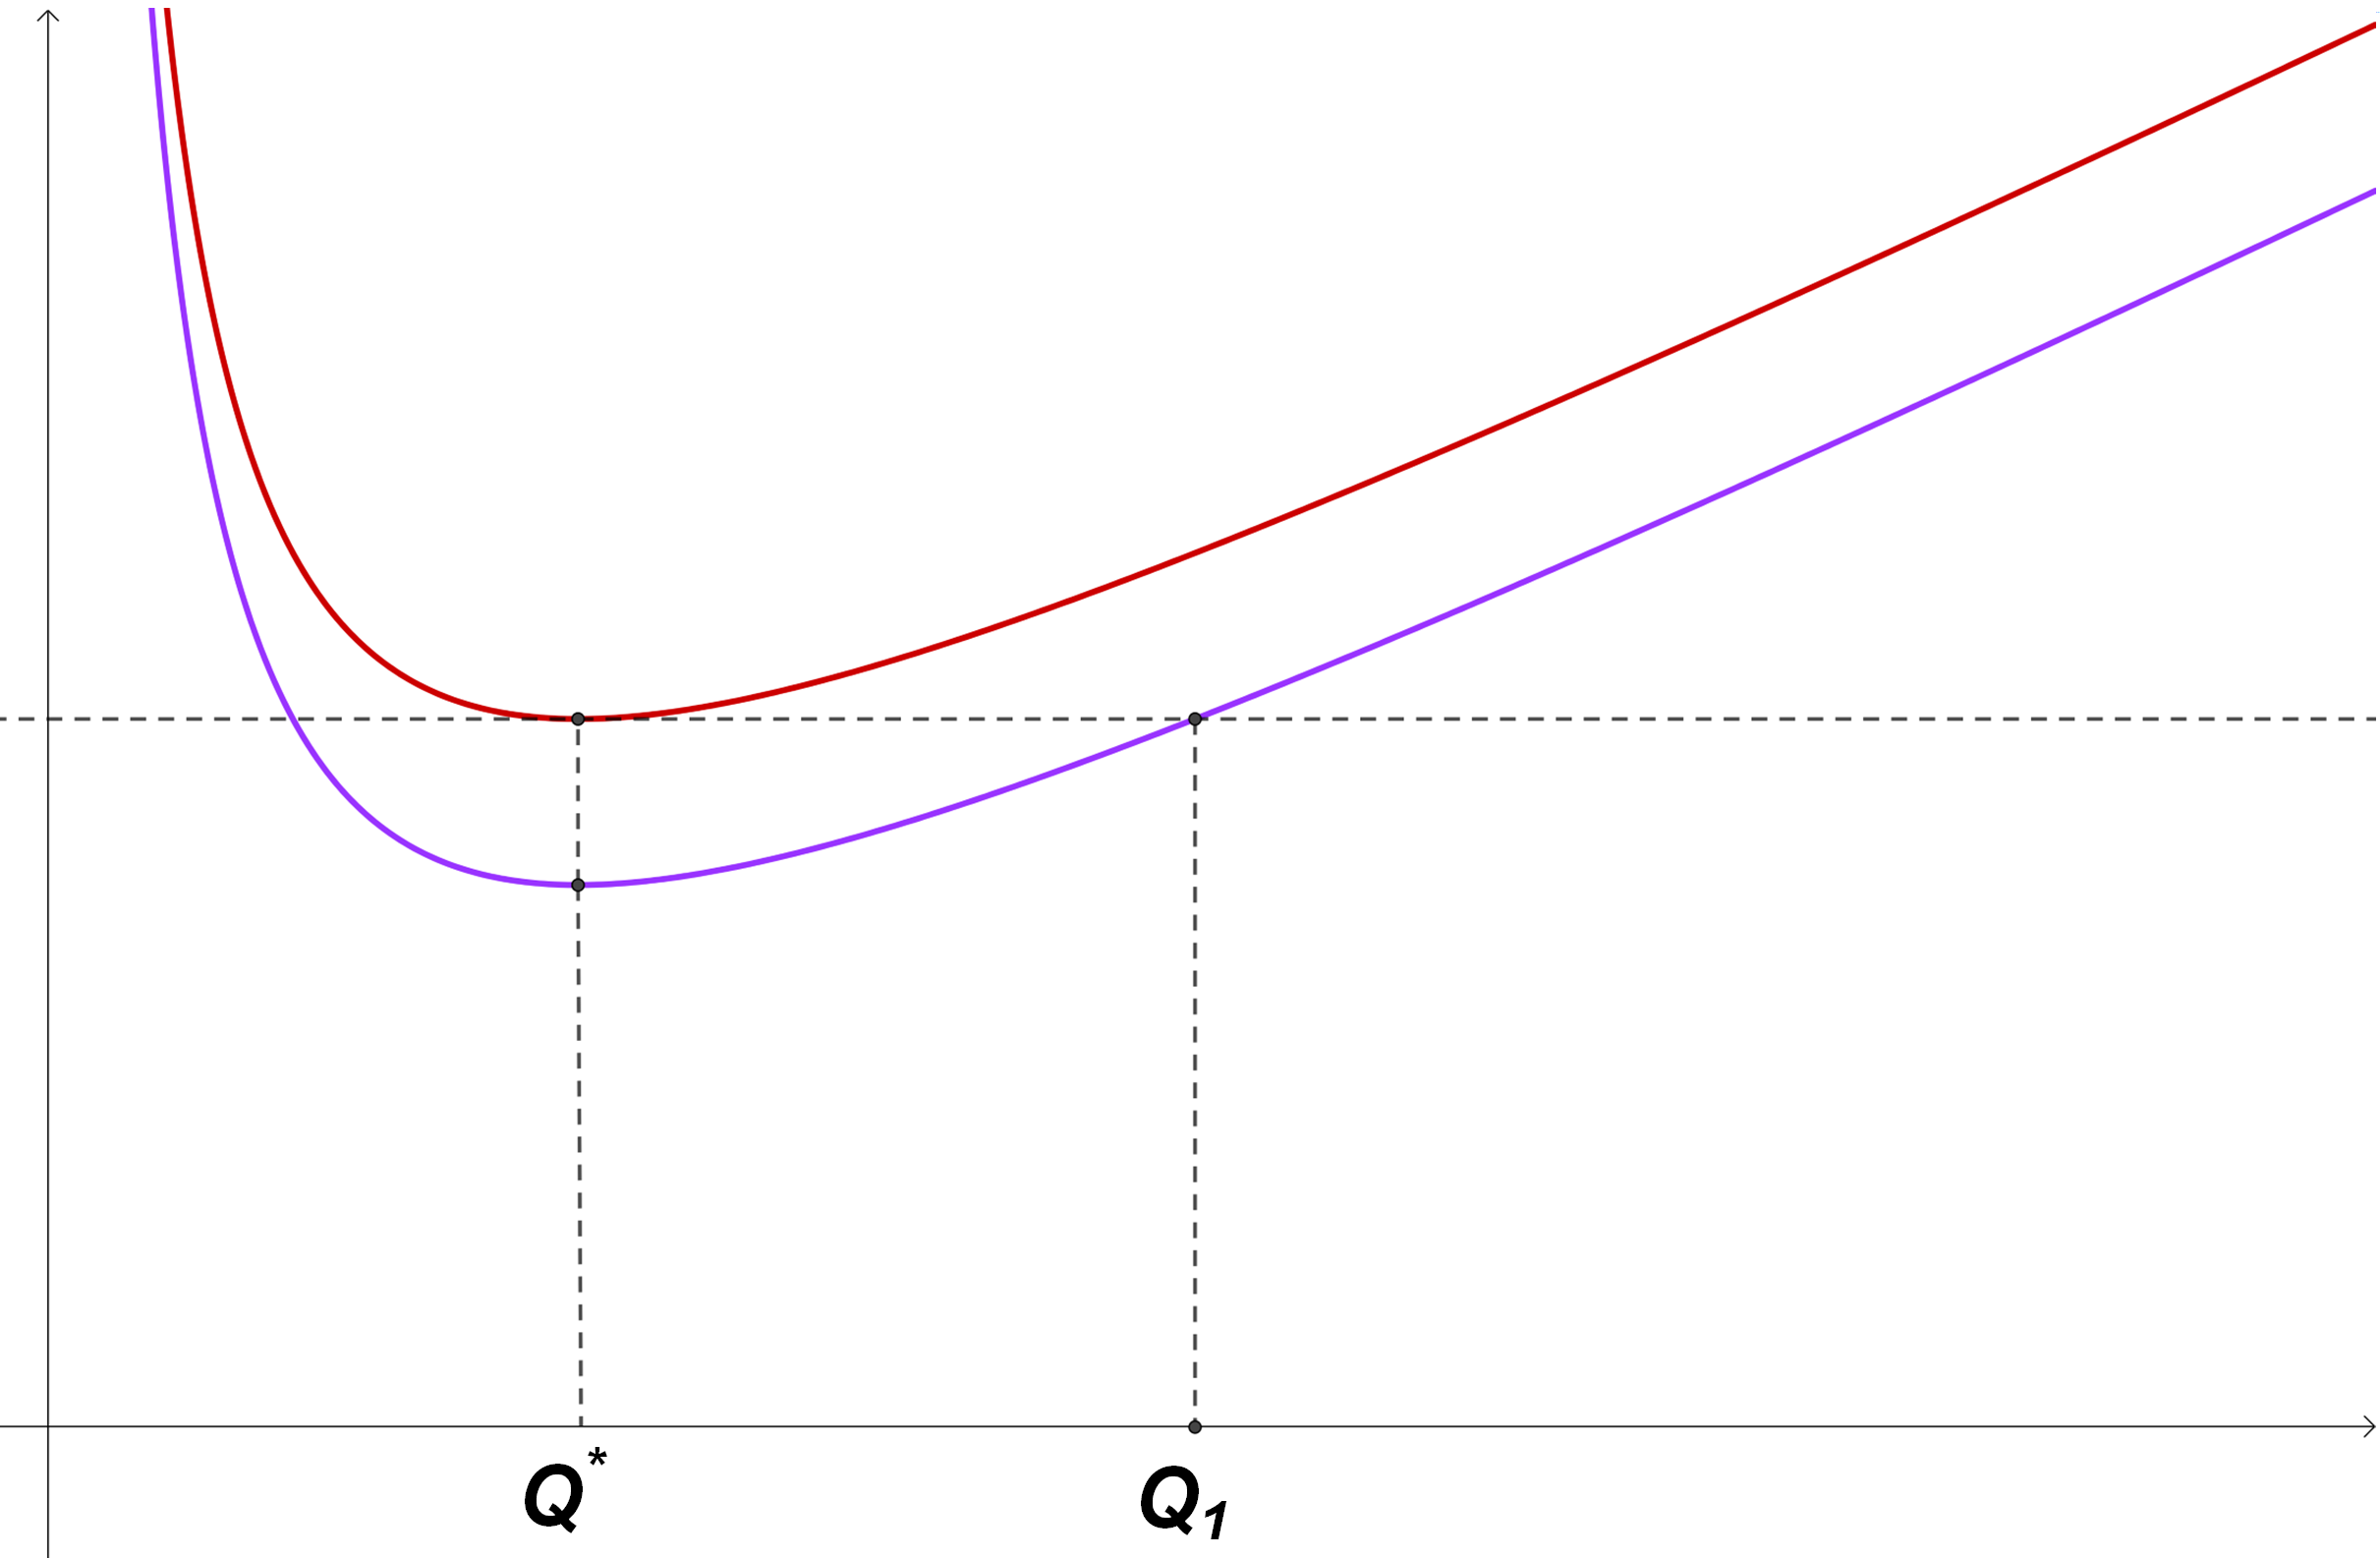
\includegraphics[width= 1\linewidth]{5}
		\caption{\small\textit{\color{toanhocdoisong}Hình $4$. Đồ thị của $T_1(Q)$ và $T_2(Q)$.}}
		\vspace*{-10pt}
	\end{figure}
	Hàm chi phí của ta sẽ có dạng:
	\begin{align*}
		T(Q) = \begin{cases}
			T_1(Q),Q \le q\\
			T_2(Q),Q > q
		\end{cases}
	\end{align*}
	Những hàm số như trên còn được gọi là hàm số liên tục theo từng đoạn. Để tìm cực tiểu của nó, ta cần xét $3$ trường hợp khác nhau.
	\vskip 0.1cm
	$\bullet$ Trường hợp $1$: $q<Q^*$.  Khi đó cực tiểu sẽ trùng với $Q=Q^*$ (Hình $5$).
	\begin{figure}[H]
		\vspace*{-5pt}
		\centering
		\captionsetup{labelformat= empty, justification=centering}
		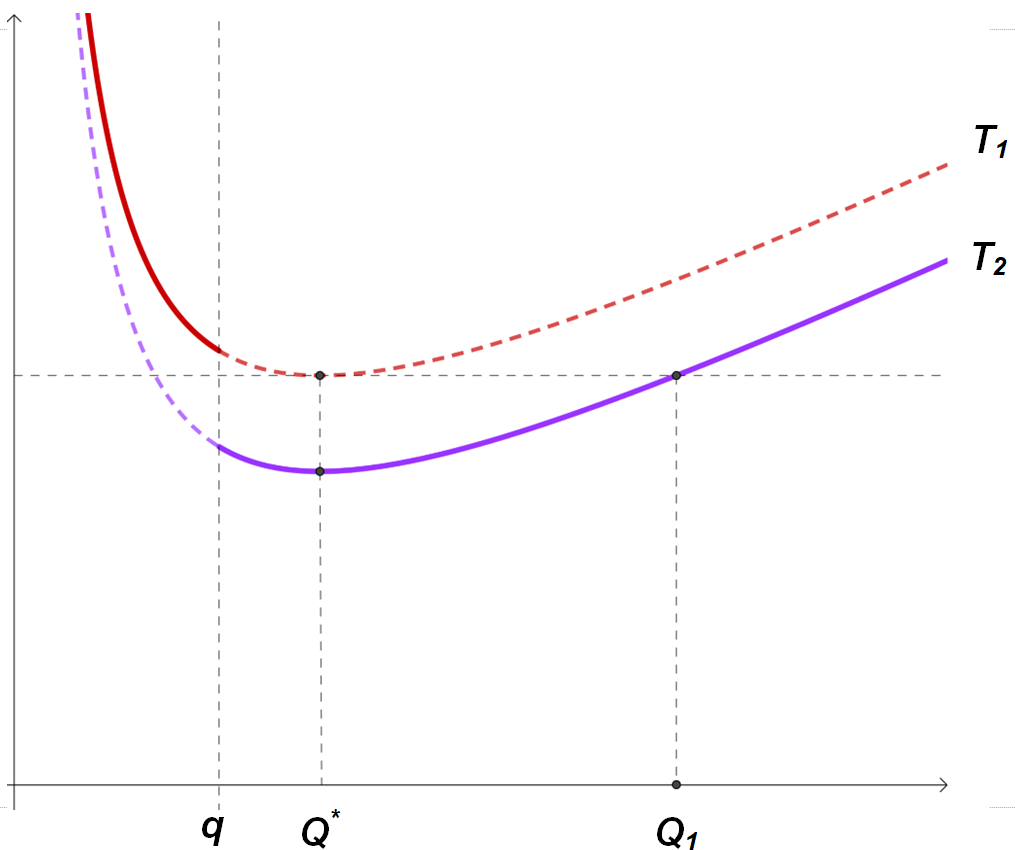
\includegraphics[width= 1\linewidth]{6}
		\caption{\small\textit{\color{toanhocdoisong}Hình $5$. Trường hợp $1$, $q<Q^*$.}}
		\vspace*{-10pt}
	\end{figure}
	$\bullet$ Trường hợp $2$: $Q^* \le q \le Q_1$. Nhìn vào Hình $6$, ta thấy cực tiểu sẽ đạt được khi $Q=q$. Ta mua hàng với số lượng nhỏ nhất để vẫn được mua với giá thấp hơn.
	\begin{figure}[H]
		\vspace*{-5pt}
		\centering
		\captionsetup{labelformat= empty, justification=centering}
		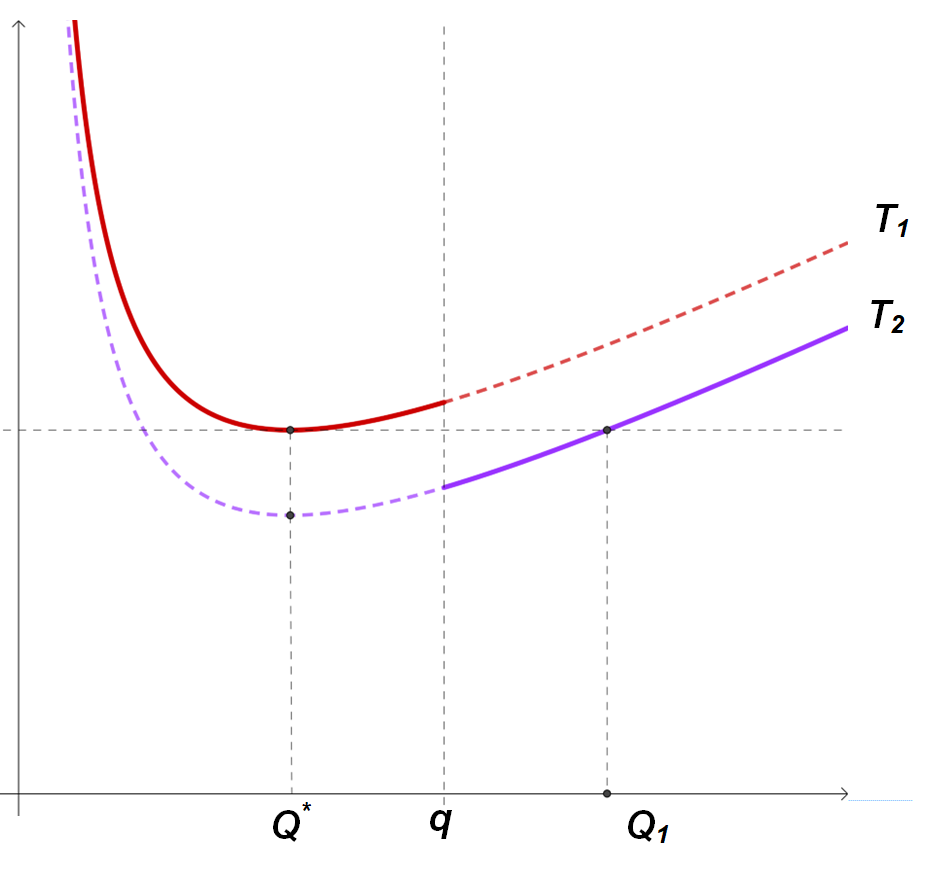
\includegraphics[width= 1\linewidth]{7}
		\caption{\small\textit{\color{toanhocdoisong}Hình $6$. Trường hợp $2$: $Q^* \le q \le Q_1$.}}
		\vspace*{-10pt}
	\end{figure}
	$\bullet$ Trường hợp $3$: $q>Q_1$. Tương tự trường hợp $1$, ta mua với số lượng $Q=Q^*$. Tuy không được hưởng chiết khấu nhưng chi phí lưu kho của ta vẫn nhỏ hơn so với việc mua nhiều để được chiết khấu.
	\begin{figure}[H]
%		\vspace*{-5pt}
		\centering
		\captionsetup{labelformat= empty, justification=centering}
		
\includegraphics[width= 1\linewidth]{8}
		\caption{\small\textit{\color{toanhocdoisong}Hình $7$. Trường hợp $3$: $q>Q_1$}}
		\vspace*{-10pt}
	\end{figure}
	Bạn đọc có thể thử tự giải cho trường hợp có nhiều hơn $2$ tầng phân khúc của giá hàng. Khi đó ta sẽ có một bài toán khảo sát hàm số liên tục từng đoạn tương đối thú vị.
	\vskip 0.1cm
	$\pmb{4.}$ \textbf{\color{toanhocdoisong}Mô hình EOQ ngẫu nhiên và bài toán sạp báo}
	\begin{figure}[H]
		\vspace*{-5pt}
		\centering
		\captionsetup{labelformat= empty, justification=centering}
		
\includegraphics[width= 1\linewidth]{9}
		\caption{\small\textit{\color{toanhocdoisong}Hình $8$. Báo ra hàng ngày có giá trị giảm nhiều vào ngày hôm sau nên việc đặt mua bao nhiêu báo cũng là một vấn đề quan trọng của các sạp báo.}}
		\vspace*{-10pt}
	\end{figure}
	Ta hãy sử dụng mô hình EOQ để nghiên cứu một bài toán phức tạp hơn. Xét một sạp báo với lượng báo $S$ được đặt vào đầu buổi sáng. Nếu báo đặt không đủ nhu cầu, ta có chi phí phạt $p$ cho một đơn vị báo bị thiếu hụt, còn nếu báo đặt bị thừa, do nó là mặt hàng có giá trị suy giảm theo thời gian ta sẽ có chi phí $h$ để lưu trữ mỗi đơn vị sang ngày hôm sau (bao gồm chi phí giữ trong kho qua đêm trừ đi giá bán rẻ hơn vào ngày hôm sau).
	\vskip 0.1cm
	Gọi $D$ là nhu cầu trong ngày và giá một đơn vị báo mua vào là $c$. Chi phí của một ngày sẽ là:
	\begin{align*}
		C(D,S) = \,&cS + p\max(0,D - S) \\
		&+ h\max(0,S-D).
	\end{align*}
	Ở đây, chi phí phạt chỉ xuất hiện khi nhu cầu nhiều hơn lượng báo ta có, còn chi phí lưu trữ chỉ xuất hiện khi lượng báo nhiều hơn nhu cầu.
	\vskip 0.1cm
	Ta lại giả sử nhu cầu $D$ là một biến ngẫu nhiên với hàm mật độ xác suất $f(x)$. Khi đó, giá trị trung bình của chi phí của ta sẽ là:
	\begin{align*}
		C(S) =\,& E\left[C(D,S)\right] \\
			=\,& cS + \int_S^\infty  {p(x - S)f(x)dx} \\
			&+ \int_0^\infty  {h(S - x)f(x)dx.} 
	\end{align*}
	Chú ý rằng cận của hai tích phân trong biểu thức này ứng với phân tích ở trên về sự xuất hiện của $p$ và $h$ theo $S$ trong mô hình: $p$ chỉ có ý nghĩa khi $D>S$ và $h$ chỉ xuất hiện khi $D<S$.
	\vskip 0.2cm
	\PIbox{Với biến ngẫu nhiên nhận các giá trị liên tục, người ta sử dụng khái niệm hàm mật độ. Xác suất để biến ngẫu nhiên $X$ với hàm mật độ $f(x)$ nằm trong khoảng $[a,b]$ sẽ là $\int_a^b{f(x)dx}$.
	}
	\vskip 0.2cm
	Đến đây ta gặp phải vấn đề làm thế nào để tìm cực trị của một hàm số có chứa tích phân! Tuy rằng các công thức giải tích đại học có thể cho ta kết quả ngay, việc sử dụng các kiến thức toán phổ thông để tìm cực trị của $C(S)$ cũng không quá khó. Ta viết lại $C(S)$ dưới dạng:
	\begin{align*}
		&C(S) \\
		= \,&cS + p\int_S^{\infty}{xf(x)dx} - pS\int_S^{\infty}{f(x)dx}\\
		 &+ hS\int_0^{S}{f(x)dx} - h\int_0^{S}{xf(x)dx}\\
		= \,&cS \!+\! p\left[G(\infty) \!-\! G(S)\right] \!-\! pS\left[F(\infty) \!-\! F(S)\right]\\
		&+ hS\left[F(S) - F(0)\right] - h\left[G(S) - G(0)\right],
	\end{align*}
	với $F$ và $G$ lần lượt là nguyên hàm của $f(x)$ và $xf(x)$.
	\vskip 0.1cm
	Ta lấy đạo hàm của $C(S)$ theo $S$, (sử dụng các công thức $\dfrac{dF(S)}{dS} = f(S)$ và $\dfrac{dG(S)}{dS} = Sf(S)$):
	\begin{align*}
		&\frac{dC(S)}{dS} \\
		= \,&c - pSf(S) - pF(\infty) + pF(S) + pSf(S) \\
		&+ hF(S) + hSf(S) - hF(0) - hSf(S)\\
		= \,&c- p\left[F(\infty) - F(S)\right] + h\left[F(S) - f(0)\right]\\
		= \,&c- p\int_S^{\infty}{f(x)dx} + h\int_0^{S}{f(x)dx}.
	\end{align*}
	Chú ý rằng ở đây ta đã sử dụng dạng ngược của công thức Newton--Leibniz: $F(b)-F(a)= \int_a^b{f(x)dx}$. Trong trường hợp các hàm số $f(x)$ và $xf(x)$ không có nguyên hàm, ta cần tính đạo hàm theo giới hạn để tính đạo hàm của tích phân có cận phụ thuộc tham biến (xem phụ lục).
	\vskip 0.1cm
	Vì $f(x)$ là hàm mật độ xác suất nên $\int_0^{\infty}{f(x)dx} = 1$ (ứng với $P(0 \le D \le \infty)=1$). Do đó:
	\begin{align*}
		\int_0^{S}{f(x)dx} + \int_S^{\infty}{f(x)dx} = \int_0^{\infty}{f(x)dx}=1.
	\end{align*}
	Thay vào biểu thức của $\dfrac{dC(S)}{dS}$ ta được:
	\begin{align*}
		&\frac{dC(S)}{dS} \\
		= \,&c- p\left(1- \int_0^{S}{f(x)dx}\right) + h\int_0^{S}{f(x)dx} \\
		= \,&(c-p) + (p+h)\int_0^{S}{f(x)dx}.
	\end{align*}
	Để tìm cực trị, ta cho biểu thức trên bằng $0$ và được:
	\begin{align*}
		(p+h)\int_0^{S}{f(x)dx} = p-c,
	\end{align*}
	hay:
	\begin{align*}
		\int_0^{S}{f(x)dx} = \frac{p-c}{p+h}
	\end{align*}
	Do đó cực trị xuất hiện ở giá trị $S^*$ sao cho:
	\begin{align*}
		F(S^*) = \frac{p-c}{p+h}.
	\end{align*}
	Ở đây ta đã chọn $F(S)$ sao cho $F(0)=0$. Khi đó $F(x)$ trở thành hàm phân phối cộng dồn cho biến ngẫu nhiên $D$. Giá trị $F(x)$ sẽ bằng với xác suất $P(D \le x)$.
	\vskip 0.1cm
	Có thể thấy, việc sử dụng nguyên hàm và các công thức có liên quan cho phép ta tìm cực trị của một hàm số có chứa tích phân chỉ sau một vài biến đổi.
	\vskip 0.1cm
	Mô hình trên cho bài toán sạp báo cũng có thể được áp dụng cho các trường hợp khác trong thực tế khi người ta cần phải tính đến việc một số loại hàng hóa không giữ nguyên giá trị nếu bị lưu kho đến giai đoạn thời gian tiếp theo. Các ví dụ thường thấy bao gồm: thực phẩm, hoa, quần áo (ví dụ quần áo mùa đông khi mùa hè sắp đến), ...
	\vskip 0.1cm
	Trong trường hợp trước khi đặt hàng, cửa hàng vẫn còn tồn một lượng hàng hóa I từ trước đó thì chi phí của ta sẽ là:
	\begin{align*}
		\overline{C}(S) = C(S) - CI.
	\end{align*}
	Nếu $I<S^*$ thì ta chỉ cần đặt một lượng hàng hóa đúng bằng $S^*-I$.
	\vskip 0.1cm
	Trong trường hợp $I\ge S^*$, ta cần xét xem $C(S)$ đồng biến hay nghịch biến trong khoảng này. Do $f(x)>0$ với mọi $x$ nên $\dfrac{dC(S)}{dS}$ tăng khi $S$ tăng. Tại $S=S^*, \dfrac{dC(S)}{dS}=0$ nên $\dfrac{dC(S)}{dS}$ sẽ $>0$ với $S>S^*$. Vì vậy, trong trường hợp này, ta không đặt thêm hàng nữa mà chỉ bán hết lượng hàng $I$ còn trong kho.
	\vskip 0.1cm
	Nếu có thêm chi phí thiết lập đơn hàng $K$ thì hàm chi phí của ta có giá trị như sau:
	\vskip 0.1cm
	$\overline{C}(S) = K + C(S) - cI$ nếu đơn hàng được đặt
	và $\overline{C}(S) = C(I)- cI$ nếu không đặt hàng mà chi bán nốt hàng trong kho.
	\begin{figure}[H]
		\vspace*{-5pt}
		\centering
		\captionsetup{labelformat= empty, justification=centering}
		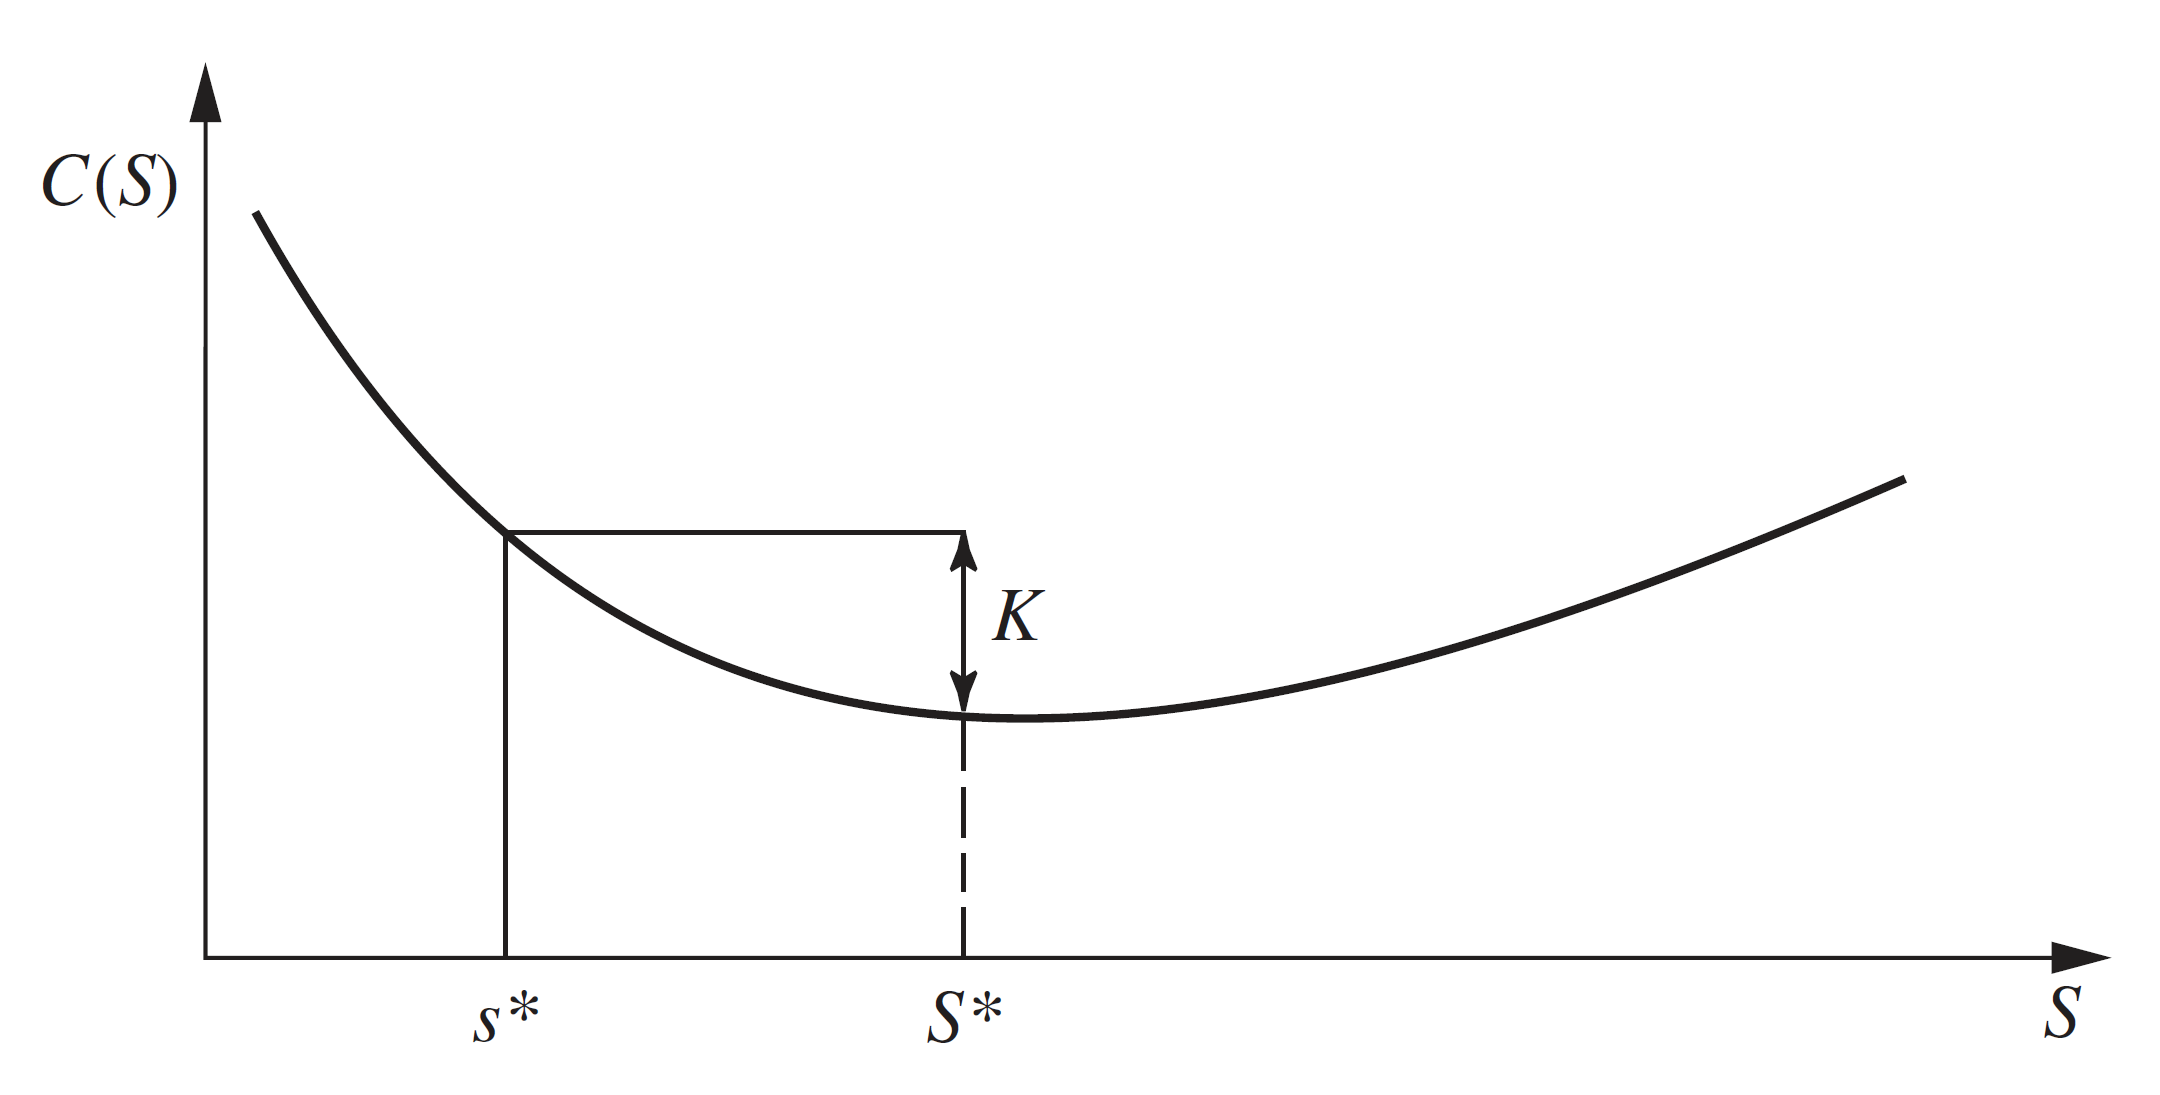
\includegraphics[width= 1\linewidth]{10}
		\caption{\small\textit{\color{toanhocdoisong}Hình $9$. Cách tìm $s^*$ khi có $S^*$.}}
		\vspace*{-10pt}
	\end{figure}
	Ta hãy xét một giá trị $s^*<S^*$ sao cho $C(s^* )=K+C(S^*)$ (giá trị $s^*>S*$ không có ý nghĩa về mặt thực tế). Trong một bài toán cụ thể, nếu đã biết được dạng của $f(x), s^*$ là hoàn toàn xác định được. 
	\vskip 0.1cm
	Phương án của ta cho trường hợp $I>0,K>0$ sẽ như sau:
	\vskip 0.1cm
	Nếu $I<s^*$ thì $C(S^* )<K+C(I)$ và ta đặt hàng với lượng hàng bằng $S^*$.
	\vskip 0.1cm
	Nếu $I \ge s^*$ thì $C(S) \le K+C(I)$ với mọi $S \ge I$ do đó ta không đặt hàng.
	\vskip 0.1cm
	$\pmb{5.}$ \textbf{\color{toanhocdoisong}Lời kết}
	\vskip 0.1cm
	Trong bài viết này, chúng ta đã thấy sự đa dạng của các bài toán có sử dụng mô hình EOQ cũng như việc ứng dụng các kỹ thuật đa dạng tìm cực trị của hàm số để cho ra nghiệm tối ưu. Các bài toán cực trị còn rất nhiều ứng dụng khác trong đời sống mà Pi sẽ trình bày với độc giả trong những số sau này.
	\vskip 0.1cm
	\textbf{\color{toanhocdoisong}Phụ lục:} Đạo hàm của tích phân có cận phụ thuộc tham biến
	\vskip 0.1cm
	Xét tích phân $I(t) = \int_{\alpha(t)}^{\beta(t)}{f(x)dx}$ với $ \alpha(t)$ và  $\beta(t)$ là các hàm khả vi theo $t$. Giả sử rằng khi $t \in [c,d]$ thì  $\alpha(t)$ và  $\beta(t)$ nhận giá trị trong $[a,b]$.
	\vskip 0.1cm
	Xét $t_0 \in [c,d]$, ta có:
	\begin{align*}
		I(t) =& \int_{\alpha(t)}^{\alpha(t_0)}{f(x)dx} + \int_{\alpha(t_0)}^{\beta(t_0)}{f(x)dx} \\
		&+ \int_{\beta(t_0)}^{\beta(t)}{f(x)dx}\\
		=& I_1(t) + I_2 + I_3(t).
	\end{align*}
	Do $I_2$ không phụ thuộc $t$ nên:
	\begin{align*}
		I'(t_0) = I_1'(t_0) + I_3'(t_0).
	\end{align*}
	Theo định nghĩa đạo hàm:
	\begin{align*}
		&I_3'(t_0)= \mathop {\lim }\limits_{t \to {t_0}} \frac{{{I_3}(t) - {I_3}({t_0})}}{{t - {t_0}}} \\
		= &\mathop {\lim }\limits_{t \to {t_0}} \frac{1}{{t \!-\! {t_0}}}\!\!\left[ \int_{\beta ({t_0})}^{\beta (t)} {f(x)dx}  \!-\! \int_{\beta ({t_0})}^{\beta ({t_0})} {f(x)dx}  \right] \\
		= &\mathop {\lim }\limits_{t \to {t_0}} \frac{1}{{t - {t_0}}}\int_{\beta ({t_0})}^{\beta (t)} {f(x)dx}
	\end{align*}
	Đến đây, ta cần dùng định lý giá trị trung bình cho tích phân: với hàm số $f(x)$ liên tục trên $[a,b]$, tồn tại giá trị $\xi \in [a,b]$ sao cho $\int_a^b{f(x)dx} = (b-a)f(\xi)$. Thật vậy, xét hàm số $f(x)$ liên tục trong khoảng $[a,b]$, khi đó tồn tại giá trị $m$ và $M$ sao cho $m \le f(x) \le M$ với mọi $x$ trong khoảng trên. Do đó:
	\begin{align*}
		\int_a^b{mdx} \le \int_a^b{f(x)dx} \le \int_a^b{Mdx},
	\end{align*}
	hay 
	\begin{align*}
		m(b-a) \le \int_a^b{f(x)dx} \le M (b-a).
	\end{align*}
	Việc này tương đương với: $\int_a^b{f(x)dx} = c(b-a), m \le c \le M$. Vì $f(x)$ là liên tục nên tồn tại giá trị $a \le \xi \le b$ sao cho $f(\xi)= c$ hay $\int_a^b{f(x)} = (b-a)f(\xi)$.
	\vskip 0.1cm
	Sử dụng định lý này cho biểu thức của $I_3'(t_0)$, ta có:
	\begin{align*}
		I_3'(t_0) &= \mathop {\lim }\limits_{t \to {t_0}} \frac{{\beta (t) - \beta ({t_0})}}{{t - {t_0}}}f(\xi ) \\
		&= \beta '({t_0})f\left( {\beta ({t_0})} \right).
	\end{align*}
	Tương tự:
	\begin{align*}
		I_1'(t_0) = - \alpha'(t_0)f\left(\alpha(t_0)\right).
	\end{align*}
	\textbf{\color{toanhocdoisong}Tài liệu tham khảo}
	\vskip 0.1cm
	[$1$] Erlenkotter, D. ($1990$). Ford Whitman Harris and the Economic Order Quantity Model. \textit{Operations Research}, $38(6)$, $937-946$. \url{https://www.jstor.org/stable/170961}
	\vskip 0.1cm
	[$2$] Hillier, F. S., \& Lieberman, G. J. ($2015$). \textit{Introduction to operations research}. Mcgraw--Hill.
	\vskip 0.1cm
	[$3$] Taha, H. A. ($2017$). \textit{Operations research: an introduction}. Pearson Education Limited.
\end{multicols}